% ======================================================================
% fig_overview -- standalone build of a figure that main.tex also draws inline.
% ----------------------------------------------------------------------
% The tikzpicture below is copied VERBATIM from main.tex, so this file and
% the inline version render identically. Build with:
%     pdflatex fig_overview.tex
% The standalone class crops the PDF to the picture's bounding box, so no
% trim/clip is ever needed in the paper.
%
% Fonts: the picture inherits times/helvet, so every glyph is Type 1 and
% embedded by pdflatex. Nothing is rasterised, so DPI does not apply.
% ======================================================================
\documentclass[border=2pt]{standalone}

\usepackage{times}
\usepackage{helvet}
\usepackage{courier}
\usepackage{amsmath}
\usepackage{amssymb}
\usepackage{xcolor}
\usepackage{pifont}
\usepackage{tikz}
\usetikzlibrary{arrows.meta,positioning}

%% ======================================================================
%% preamble-figures.tex
%% ----------------------------------------------------------------------
%% Every definition the figures need, kept identical to main.tex's preamble.
%% Shared by the standalone builds in this folder; main.tex carries its own
%% copy so that the submitted source stays a single .tex file.
%% ======================================================================

\providecommand{\method}{\textsc{ESV}}

%% --- comparison-table glyphs (fig_trap uses \yes / \no) ---------------
\definecolor{okgreen}{RGB}{0,122,87}
\definecolor{okred}{RGB}{176,42,32}
\providecommand{\yes}{\textcolor{okgreen}{\ding{51}}}
\providecommand{\no}{\textcolor{okred}{\ding{55}}}
\providecommand{\na}{\textcolor{black!45}{--}}

%% --- figure fills, shaded by what each step costs ---------------------
\definecolor{cshared}{RGB}{226,226,226}
\definecolor{ccode}{RGB}{205,228,243}
\definecolor{ccall}{RGB}{252,230,192}
\definecolor{ccallb}{RGB}{191,118,0}
\definecolor{cout}{RGB}{206,238,227}
\definecolor{ctrap}{RGB}{250,222,218}

%% --- plot colours and markers -----------------------------------------
%% Marker shapes are core TikZ nodes, so every glyph is vector and uses the
%% document's Type 1 text fonts: no Type 3 subsets, no raster, nothing to crop.
\definecolor{pblue}{RGB}{31,97,160}
\definecolor{pgreen}{RGB}{0,122,87}
\definecolor{pgrey}{RGB}{95,95,95}
\providecommand{\mkopensq}[2]{\node[draw=#2,fill=white,line width=.6pt,rectangle,inner sep=1.5pt] at #1 {};}
\providecommand{\mkfillsq}[2]{\node[draw=#2,fill=#2,rectangle,inner sep=1.5pt] at #1 {};}
\providecommand{\mkopenci}[2]{\node[draw=#2,fill=white,line width=.6pt,circle,inner sep=1.5pt] at #1 {};}
\providecommand{\mkfillci}[2]{\node[draw=#2,fill=#2,circle,inner sep=1.5pt] at #1 {};}
%% #1 x, #2 centre, #3 half-width of the interval, #4 colour (needs x=1cm)
\providecommand{\ebar}[4]{%
  \draw[#4,line width=.5pt] (#1,{#2-#3}) -- (#1,{#2+#3});
  \draw[#4,line width=.5pt] ({#1-0.055},{#2-#3}) -- ({#1+0.055},{#2-#3});
  \draw[#4,line width=.5pt] ({#1-0.055},{#2+#3}) -- ({#1+0.055},{#2+#3});}

%% --- \cost is used inside the three schematic figures -----------------
\providecommand{\cost}{\scriptsize}


\begin{document}
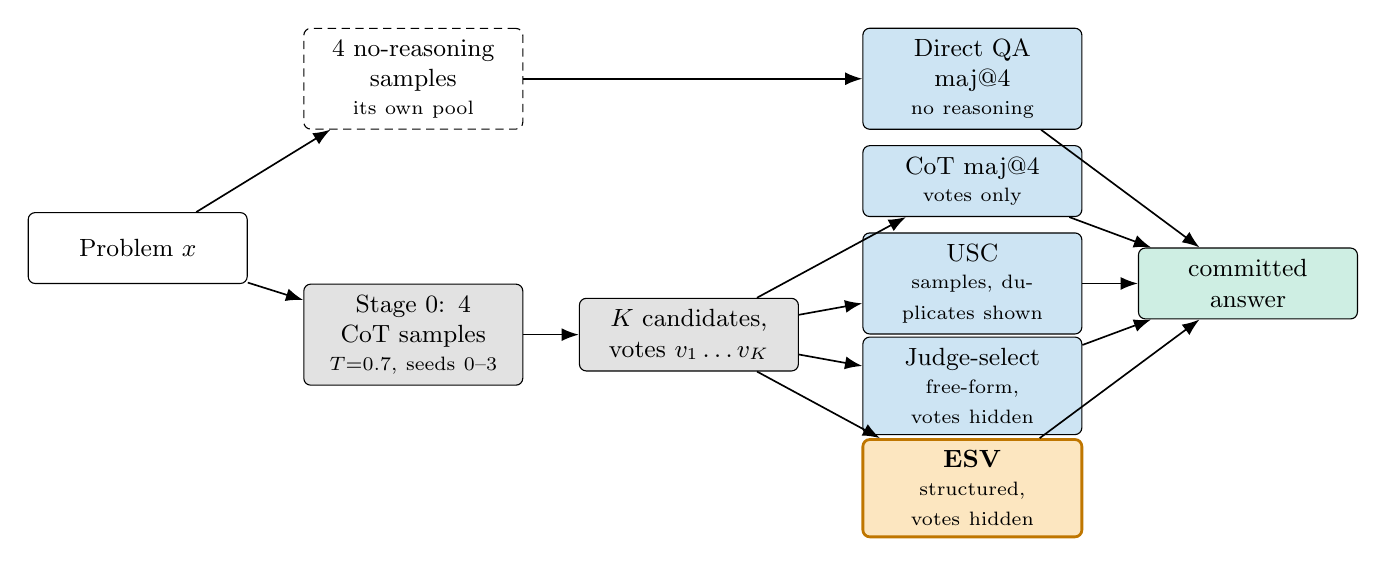
\begin{tikzpicture}[
  font=\small,
  %% text width is fixed, so no box can grow into a neighbour's gap
  base/.style={draw, rounded corners=2.5pt, align=center, inner sep=4pt,
               text width=25mm, minimum height=9mm},
  input/.style={base, fill=white},
  shared/.style={base, fill=cshared},
  own/.style={base, fill=white, densely dashed},
  sel/.style={base, fill=ccode},
  ours/.style={base, fill=ccall, draw=ccallb, line width=1pt},
  outbox/.style={base, fill=cout},
  ar/.style={-{Latex[length=2.2mm]}, semithick},
  cost/.style={font=\scriptsize},
]
\node[input]  (prob)  at (0,-0.2)     {Problem $x$};
\node[own]    (dpool) at (3.5,1.95)   {$4$ no-reasoning samples\\[-1pt]{\cost its own pool}};
\node[shared] (pool)  at (3.5,-1.3)   {Stage~0: $4$ CoT samples\\[-1pt]{\cost $T{=}0.7$, seeds $0$--$3$}};
\node[shared] (cands) at (7.0,-1.3)   {$K$ candidates, votes $v_1 \dots v_K$};

\node[sel]    (dqa)   at (10.6,1.95)  {Direct QA maj@4\\[-1pt]{\cost no reasoning}};
\node[sel]    (maj)   at (10.6,0.65)  {CoT maj@4\\[-1pt]{\cost votes only}};
\node[sel]    (usc)   at (10.6,-0.65) {USC\\[-1pt]{\cost samples, duplicates shown}};
\node[sel]    (jud)   at (10.6,-1.95) {Judge-select\\[-1pt]{\cost free-form, votes hidden}};
\node[ours]   (esv)   at (10.6,-3.25) {\textbf{\method{}}\\[-1pt]{\cost structured, votes hidden}};

\node[outbox] (ans)   at (14.1,-0.65) {committed answer};

\draw[ar] (prob)  -- (dpool);
\draw[ar] (prob)  -- (pool);
\draw[ar] (dpool) -- (dqa);
\draw[ar] (pool)  -- (cands);
\draw[ar] (cands) -- (maj);
\draw[ar] (cands) -- (usc);
\draw[ar] (cands) -- (jud);
\draw[ar] (cands) -- (esv);
\draw[ar] (dqa)   -- (ans);
\draw[ar] (maj)   -- (ans);
\draw[ar] (usc)   -- (ans);
\draw[ar] (jud)   -- (ans);
\draw[ar] (esv)   -- (ans);
\end{tikzpicture}
\end{document}
